\documentclass[
	ngerman,
	toc=listof, % Abbildungsverzeichnis sowie Tabellenverzeichnis in das Inhaltsverzeichnis aufnehmen
	toc=bibliography, % Literaturverzeichnis in das Inhaltsverzeichnis aufnehmen
	footnotes=multiple, % Trennen von direkt aufeinander folgenden Fußnoten
	parskip=half, % vertikalen Abstand zwischen Absätzen verwenden anstatt horizontale Einrückung von Folgeabsätzen
	numbers=noendperiod % Den letzten Punkt nach einer Nummerierung entfernen (nach DIN 5008)
]{scrartcl}
\pdfminorversion=5 % erlaubt das Einfügen von pdf-Dateien bis Version 1.7, ohne eine Fehlermeldung zu werfen (keine Garantie für fehlerfreies Einbetten!)

% Dokumenteninformationen ----------------------------------------------------
\newcommand{\titel}{Domainanalyse}
\newcommand{\untertitel}{Studienarbeit \semester}
\newcommand{\kompletterTitel}{\titel{} \\ \untertitel}
\newcommand{\datum}{\today}

\newcommand{\vorlagenOrdner}{../../99_Vorlagen} % Falls im Unterordner ../ vorne hinzufügen

\newcommand{\betriebLogo}{\vorlagenOrdner/Bilder/logo}

% Konfiguration -------------------------------------------------------------
\newcommand{\autoren}{
    \author{
        Schmid, Mike\\
        \texttt{sgschwin@hsr.ch}
        \and
        Schlatter, Janik\\
        \texttt{jschlatt@hsr.ch}
    }
}

\newcommand{\betreuer}{
    Stettler Beat\\
    \scriptsize \texttt{\url{beat.stettler@hsr.ch}}
    \normalsize
}

\newcommand{\schmid}{
    Mike Schmid\\
    \url{mschmid@hsr.ch}
    \normalsize
}

\newcommand{\schlatter}{
    Janik Schlatter\\
    \scriptsize \url{jschlatt@hsr.ch}
    \normalsize
}

\newcommand{\autorenNamen}{
    M. Schmid, J. Schlatter
}

\newcommand{\semester}{FS-2020}
\newcommand{\betriebName}{\textsc{HSR} Hochschule für Technik Rapperswil} % Metadaten zu diesem Dokument (Autor usw.)
% !TEX root = ../Projektdokumentation.tex

% Anpassung an Landessprache ---------------------------------------------------
\usepackage[english, main=ngerman]{babel} % \selectlanguage{english} if  needed

% Umlaute ----------------------------------------------------------------------
%   Umlaute/Sonderzeichen wie äüöß direkt im Quelltext verwenden (CodePage).
%   Erlaubt automatische Trennung von Worten mit Umlauten.
% ------------------------------------------------------------------------------
\usepackage[T1]{fontenc}
\usepackage[utf8]{inputenc}
\usepackage{textcomp} % Euro-Zeichen etc.

% Schrift ----------------------------------------------------------------------
\usepackage{lmodern} % bessere Fonts
\usepackage{relsize} % Schriftgröße relativ festlegen

% Tabellen ---------------------------------------------------------------------
\PassOptionsToPackage{table}{xcolor}
\usepackage{tabularx}
\usepackage{tabulary}
\usepackage{booktabs}
\usepackage{makecell}
\usepackage[table,xcdraw]{xcolor}
% für lange Tabellen
\usepackage{longtable}
\usepackage{array}
\usepackage{ragged2e}
\usepackage{lscape}
% Multi Columns
\usepackage{multicol}

% Grafiken ---------------------------------------------------------------------
\usepackage[dvips,final]{graphicx} % Einbinden von JPG-Grafiken ermöglichen
\usepackage{graphics} % keepaspectratio
\usepackage{floatflt} % zum Umfließen von Bildern
\graphicspath{{Bilder/}} % hier liegen die Bilder des Dokuments

% Sonstiges --------------------------------------------------------------------
\usepackage[titles]{tocloft} % Inhaltsverzeichnis DIN 5008 gerecht einrücken
\usepackage{enumitem} % anpassbare Enumerates/Itemizes
\usepackage{xspace} % sorgt dafür, dass Leerzeichen hinter parameterlosen Makros nicht als Makroendezeichen interpretiert werden

\usepackage{makeidx} % für Index-Ausgabe mit \printindex
\usepackage[printonlyused]{acronym} % es werden nur benutzte Definitionen aufgelistet

% Einfache Definition der Zeilenabstände und Seitenränder etc.
\usepackage{setspace}
\usepackage{geometry}

% Symbolverzeichnis
\usepackage[intoc]{nomencl}
\let\abbrev\nomenclature
\renewcommand{\nomname}{Abkürzungsverzeichnis}
\setlength{\nomlabelwidth}{.25\hsize}
\renewcommand{\nomlabel}[1]{#1 \dotfill}
\setlength{\nomitemsep}{-\parsep}

\usepackage{varioref} % Elegantere Verweise. „auf der nächsten Seite“
\usepackage{url} % URL verlinken, lange URLs umbrechen etc.

\usepackage{chngcntr} % fortlaufendes Durchnummerieren der Fußnoten
% \usepackage[perpage]{footmisc} % Alternative: Nummerierung der Fußnoten auf jeder Seite neu

\usepackage{ifthen} % bei der Definition eigener Befehle benötigt
\usepackage{todonotes} % definiert u.a. die Befehle \todo und \listoftodos
\usepackage[square]{natbib} % wichtig für korrekte Zitierweise

% PDF-Optionen -----------------------------------------------------------------
\usepackage{pdfpages}
\pdfminorversion=5 % erlaubt das Einfügen von pdf-Dateien bis Version 1.7, ohne eine Fehlermeldung zu werfen (keine Garantie für fehlerfreies Einbetten!)
\usepackage[
    bookmarks,
    bookmarksnumbered,
    bookmarksopen=true,
    bookmarksopenlevel=1,
    colorlinks=true,
% diese Farbdefinitionen zeichnen Links im PDF farblich aus
    linkcolor=AOBlau, % einfache interne Verknüpfungen
    anchorcolor=AOBlau,% Ankertext
    citecolor=AOBlau, % Verweise auf Literaturverzeichniseinträge im Text
    filecolor=AOBlau, % Verknüpfungen, die lokale Dateien öffnen
    menucolor=AOBlau, % Acrobat-Menüpunkte
    urlcolor=AOBlau,
% diese Farbdefinitionen sollten für den Druck verwendet werden (alles schwarz)
    %linkcolor=black, % einfache interne Verknüpfungen
    %anchorcolor=black, % Ankertext
    %citecolor=black, % Verweise auf Literaturverzeichniseinträge im Text
    %filecolor=black, % Verknüpfungen, die lokale Dateien öffnen
    %menucolor=black, % Acrobat-Menüpunkte
    %urlcolor=black,
%
    %backref, % Quellen werden zurück auf ihre Zitate verlinkt
    pdftex,
    plainpages=false, % zur korrekten Erstellung der Bookmarks
    pdfpagelabels=true, % zur korrekten Erstellung der Bookmarks
    hypertexnames=false, % zur korrekten Erstellung der Bookmarks
    linktocpage % Seitenzahlen anstatt Text im Inhaltsverzeichnis verlinken
]{hyperref}
% Befehle, die Umlaute ausgeben, führen zu Fehlern, wenn sie hyperref als Optionen übergeben werden
\hypersetup{
    pdftitle={\titel -- \untertitel},
    pdfauthor={\autoren},
    pdfcreator={\autoren},
    pdfsubject={\titel -- \untertitel},
    pdfkeywords={\titel -- \untertitel},
}


% zum Einbinden von Programmcode -----------------------------------------------
\usepackage{listings}
\usepackage{xcolor}
\usepackage{beramono}
% Pseudocode
\usepackage{algorithmic}
\usepackage[linesnumbered,ruled]{algorithm2e}

\definecolor{hellgelb}{rgb}{1,1,0.9}
\definecolor{colKeys}{rgb}{0,0,1}
\definecolor{colIdentifier}{rgb}{0,0,0}
\definecolor{colComments}{rgb}{0,0.5,0}
\definecolor{colString}{rgb}{1,0,0}
\definecolor{bluekeywords}{rgb}{0,0,1}
\definecolor{greencomments}{rgb}{0,0.5,0}
\definecolor{redstrings}{rgb}{0.64,0.08,0.08}
\definecolor{xmlcomments}{rgb}{0.5,0.5,0.5}
\definecolor{types}{rgb}{0.17,0.57,0.68}
\definecolor{DarkPurple}{rgb}{0.4, 0.1, 0.4}
\definecolor{DarkCyan}{rgb}{0.0, 0.5, 0.4}
\definecolor{LightLime}{rgb}{0.3, 0.5, 0.4}
\definecolor{Blue}{rgb}{0.0, 0.0, 1.0}
\definecolor{AOBlau}{rgb}{0, 0.28, 0.56}
% Tabellenfärbung:
\definecolor{heading}{rgb}{0.64,0.78,0.86}
\definecolor{odd}{rgb}{0.9,0.9,0.9}

\lstset{
    float=hbp,
	basicstyle=\footnotesize,
    identifierstyle=\color{colIdentifier},
    keywordstyle=\color{colKeys},
    stringstyle=\color{colString},
    commentstyle=\color{colComments},
    backgroundcolor=\color{hellgelb},
    columns=flexible,
    tabsize=2,
    frame=single,
    extendedchars=true,
    showspaces=false,
    showstringspaces=false,
    numbers=left,
    numberstyle=\tiny,
    breaklines=true,
    breakautoindent=true,
	captionpos=b,
}
\lstdefinestyle{visual-studio-style}{
	language=[Sharp]C,
	columns=flexible,
	showstringspaces=false,
	basicstyle=\footnotesize\ttfamily, 
	commentstyle=\color{greencomments},
	morekeywords={partial, var, value, get, set},
	keywordstyle=\bfseries\color{bluekeywords},
	stringstyle=\color{redstrings},
	breaklines=true,
	breakatwhitespace=true,
	tabsize=4,
	numbers=left,
	numberstyle=\tiny\color{black},
	frame=lines,
	showspaces=false,
	showtabs=false,
	escapeinside={£}{£},
}
\lstdefinestyle{eclipse-style}{
	language=Java,  
	columns=flexible,
	showstringspaces=false,     
	basicstyle=\footnotesize\ttfamily, 
	keywordstyle=\bfseries\color{DarkPurple},
	commentstyle=\color{LightLime},
	stringstyle=\color{Blue}, 
	escapeinside={£}{£}, % latex scope within code      
	breaklines=true,
	breakatwhitespace=true,
	showspaces=false,
	showtabs=false,
	tabsize=4,
	morekeywords={length},
	numbers=left,
	numberstyle=\tiny\color{black},
	frame=lines,
}
\lstset{style=eclipse-style}
\lstdefinelanguage{cs}{
	sensitive=false,
	morecomment=[l]{//},
	morecomment=[s]{/*}{*/},
	morestring=[b]",
	morekeywords={
		abstract,event,new,struct,as,explicit,null,switch
		base,extern,object,this,bool,false,operator,throw,
		break,finally,out,true,byte,fixed,override,try,
		case,float,params,typeof,catch,for,private,uint,
		char,foreach,protected,ulong,checked,goto,public,unchecked,
		class,if,readonly,unsafe,const,implicit,ref,ushort,
		continue,in,return,using,decimal,int,sbyte,virtual,
		default,interface,sealed,volatile,delegate,internal,short,void,
		do,is,sizeof,while,double,lock,stackalloc,
		else,long,static,enum,namespace,string},
}
\lstdefinelanguage{natural}{
	sensitive=false,
	morecomment=[l]{/*},
	morestring=[b]",
	morestring=[b]',
	alsodigit={-,*},
	morekeywords={
		DEFINE,DATA,LOCAL,END-DEFINE,WRITE,CALLNAT,PARAMETER,USING,
		IF,NOT,END-IF,ON,*ERROR-NR,ERROR,END-ERROR,ESCAPE,ROUTINE,
		PERFORM,SUBROUTINE,END-SUBROUTINE,CONST,END-FOR,END,FOR,RESIZE,
		ARRAY,TO,BY,VALUE,RESET,COMPRESS,INTO,EQ},
}
\lstdefinelanguage{php}{
	sensitive=false,
	morecomment=[l]{/*},
	morestring=[b]",
	morestring=[b]',
	alsodigit={-,*},
	morekeywords={
		abstract,and,array,as,break,case,catch,cfunction,class,clone,const,
		continue,declare,default,do,else,elseif,enddeclare,endfor,endforeach,
		endif,endswitch,endwhile,extends,final,for,foreach,function,global,
		goto,if,implements,interface,instanceof,namespace,new,old_function,or,
		private,protected,public,static,switch,throw,try,use,var,while,xor
		die,echo,empty,exit,eval,include,include_once,isset,list,require,
		require_once,return,print,unset},
}
 % verwendete Packages
% !TEX root = ../Projektdokumentation.tex

% Seitenränder -----------------------------------------------------------------
\setlength{\topskip}{\ht\strutbox} % behebt Warnung von geometry
\geometry{
	a4paper,
	left=20mm,
	right=20mm,
	top=25mm,
	bottom=40mm
}

\usepackage[
	automark, % Kapitelangaben in Kopfzeile automatisch erstellen
	headsepline, % Trennlinie unter Kopfzeile
	% footsepline, % Trennlinie oberhalb Fusszeile
	ilines % Trennlinie linksbündig ausrichten
]{scrpage2}

% Kopf- und Fußzeilen ----------------------------------------------------------
\pagestyle{scrheadings}
% chapterpagestyle gibt es nicht in scrartcl
%\renewcommand{\chapterpagestyle}{scrheadings}
\clearscrheadfoot

% Kopfzeile
\renewcommand{\headfont}{\normalfont} % Schriftform der Kopfzeile
\ihead{\large{\textsc{\titel}}\\ \small{\untertitel} \\[2ex] \textit{\headmark}}
\chead{}
%\ohead{\includegraphics[scale=0.125]{\betriebLogo}}
\setlength{\headheight}{20mm} % Höhe der Kopfzeile
%\setheadwidth[0pt]{textwithmarginpar} % Kopfzeile über den Text hinaus verbreitern (falls Logo den Text überdeckt)

% Fußzeile
\ifoot{\autorenNamen}
\cfoot{}
\ofoot{\pagemark}

% Überschriften nach DIN 5008 in einer Fluchtlinie
% ------------------------------------------------------------------------------

% Abstand zwischen Nummerierung und Überschrift definieren
% > Schön wäre hier die dynamische Berechnung des Abstandes in Abhängigkeit
% > der Verschachtelungstiefe des Inhaltsverzeichnisses
\newcommand{\headingSpace}{1.5cm}

% Abschnittsüberschriften im selben Stil wie beim Inhaltsverzeichnis einrücken
\renewcommand*{\othersectionlevelsformat}[3]{
  \makebox[\headingSpace][l]{#3\autodot}
}

% Für die Einrückung wird das Paket tocloft benötigt
%\cftsetindents{chapter}{0.0cm}{\headingSpace}
\cftsetindents{section}{0.0cm}{\headingSpace}
\cftsetindents{subsection}{0.0cm}{\headingSpace}
\cftsetindents{subsubsection}{0.0cm}{\headingSpace}
\cftsetindents{figure}{0.0cm}{\headingSpace}
\cftsetindents{table}{0.0cm}{\headingSpace}

% Allgemeines
% ------------------------------------------------------------------------------

\onehalfspacing % Zeilenabstand 1,5 Zeilen
\frenchspacing % erzeugt ein wenig mehr Platz hinter einem Punkt

% Schusterjungen und Hurenkinder vermeiden
\clubpenalty = 10000
\widowpenalty = 10000
\displaywidowpenalty = 10000

% Quellcode-Ausgabe formatieren
\lstset{numbers=left, numberstyle=\tiny, numbersep=5pt, breaklines=true}
\lstset{emph={square}, emphstyle=\color{red}, emph={[2]root,base}, emphstyle={[2]\color{blue}}}

\counterwithout{footnote}{section} % Fußnoten fortlaufend durchnummerieren
\setcounter{tocdepth}{\subsubsectionlevel} % im Inhaltsverzeichnis werden die Kapitel bis zum Level der subsubsection übernommen
\setcounter{secnumdepth}{\subsubsectionlevel} % Kapitel bis zum Level der subsubsection werden nummeriert

% Aufzählungen anpassen
\renewcommand{\labelenumi}{\arabic{enumi}.}
\renewcommand{\labelenumii}{\arabic{enumi}.\arabic{enumii}.}
\renewcommand{\labelenumiii}{\arabic{enumi}.\arabic{enumii}.\arabic{enumiii}}
 % Definitionen zum Aussehen der Seiten
% !TEX root = ../Projektdokumentation.tex

% Abkürzungen, ggfs. mit korrektem Leerraum
\newcommand{\bs}{$\backslash$\xspace}
\newcommand{\bspw}{bspw.\xspace}
\newcommand{\bzw}{bzw.\xspace}
\newcommand{\ca}{ca.\xspace}
\newcommand{\dahe}{\mbox{d.\,h.}\xspace}
\newcommand{\etc}{etc.\xspace}
\newcommand{\eur}[1]{\mbox{#1\,\texteuro}\xspace}
\newcommand{\evtl}{evtl.\xspace}
\newcommand{\ggfs}{ggfs.\xspace}
\newcommand{\Ggfs}{Ggfs.\xspace}
\newcommand{\gqq}[1]{\glqq{}#1\grqq{}}
\newcommand{\inkl}{inkl.\xspace}
\newcommand{\insb}{insb.\xspace}
\newcommand{\ua}{\mbox{u.\,a.}\xspace}
\newcommand{\usw}{usw.\xspace}
\newcommand{\Vgl}{Vgl.\xspace}
\newcommand{\zB}{\mbox{z.\,B.}\xspace}

% Befehle für häufig anfallende Aufgaben
\newcommand{\Abbildung}[1]{\autoref{fig:#1}}
\newcommand{\Anhang}[1]{\appendixname{}~\ref{#1}: \nameref{#1} \vpageref{#1}}
\newcommand{\includegraphicsKeepAspectRatio}[2]{\includegraphics[width=#2\textwidth,height=#2\textheight,keepaspectratio]{#1}}
\newcommand{\Zitat}[2][\empty]{\ifthenelse{\equal{#1}{\empty}}{\citep{#2}}{\citep[#1]{#2}}}
\newcommand{\Autor}[1]{\textsc{#1}} % zum Ausgeben von Autoren
\newcommand{\itemd}[2]{\item{\textbf{#1}}\\{#2}} % erzeugt ein Listenelement mit fetter Überschrift

% einfaches Wechseln der Schrift, z.B.: \changefont{cmss}{sbc}{n}
\newcommand{\changefont}[3]{\fontfamily{#1} \fontseries{#2} \fontshape{#3} \selectfont}

% Verwendung analog zu \includegraphics
\newlength{\myx} % Variable zum Speichern der Bildbreite
\newlength{\myy} % Variable zum Speichern der Bildhöhe
\newcommand\includegraphicstotab[2][\relax]{%
% Abspeichern der Bildabmessungen
\settowidth{\myx}{\includegraphics[{#1}]{#2}}%
\settoheight{\myy}{\includegraphics[{#1}]{#2}}%
% das eigentliche Einfügen
\parbox[c][1.1\myy][c]{\myx}{%
\includegraphics[{#1}]{#2}}%
}

% verschiedene Befehle um Wörter semantisch auszuzeichnen ----------------------
\newcommand{\Index}[2][\empty]{\ifthenelse{\equal{#1}{\empty}}{\index{#2}#2}{\index{#1}#2}}
\newcommand{\Fachbegriff}[2][\empty]{\ifthenelse{\equal{#1}{\empty}}{\textit{\Index{#2}}}{\textit{\Index[#1]{#2}}}}
\newcommand{\NeuerBegriff}[2][\empty]{\ifthenelse{\equal{#1}{\empty}}{\textbf{\Index{#2}}}{\textbf{\Index[#1]{#2}}}}

\newcommand{\Ausgabe}[1]{\texttt{#1}}
\newcommand{\Eingabe}[1]{\texttt{#1}}
\newcommand{\Code}[1]{\texttt{#1}}
\newcommand{\Datei}[1]{\texttt{#1}}

\newcommand{\Assembly}[1]{\textsf{#1}}
\newcommand{\Klasse}[1]{\textsf{#1}}
\newcommand{\Methode}[1]{\textsf{#1}}
\newcommand{\Attribut}[1]{\textsf{#1}}

\newcommand{\Datentyp}[1]{\textsf{#1}}
\newcommand{\XMLElement}[1]{\textsf{#1}}
\newcommand{\Webservice}[1]{\textsf{#1}}

\newcommand{\Refactoring}[1]{\Fachbegriff{#1}}
\newcommand{\CodeSmell}[1]{\Fachbegriff{#1}}
\newcommand{\Metrik}[1]{\Fachbegriff{#1}}
\newcommand{\DesignPattern}[1]{\Fachbegriff{#1}}

\newcommand{\muss}[1]{\textcolor{red}{#1}}
\newcommand{\soll}[1]{\textcolor{orange}{#1}}
\newcommand{\kann}[1]{\textcolor{blue}{#1}}

\newcommand{\success}[1]{\textcolor{greencomments}{#1}}
\newcommand{\fail}[1]{\textcolor{red}{#1}} % eigene allgemeine Befehle, die z.B. die Arbeit mit LaTeX erleichtern

\begin{document}

% Deckblatt ------------------------------------------------------------------
\phantomsection
\thispagestyle{plain}
\pdfbookmark[1]{Deckblatt}{deckblatt}
\begin{titlepage}
    \begin{center}
        \includegraphics[scale=1.5]{\betriebLogo}\\[10ex]

        \rule{\linewidth}{0.5mm}\\[2ex]
        {\huge \bfseries  \titel }\\[2ex]
        {\LARGE \untertitel }\\[2ex]
        {\large \datum}\\
        \rule{\linewidth}{0.5mm}\\[10ex]

        \begin{minipage}[t]{0.4\textwidth}
            \begin{flushleft} 
                \large \emph{Autoren:}\\
                    \large Mike \textsc{Schmid}\\
                    \scriptsize \texttt{mike.schmid@hsr.ch}\\[1ex]
                    \large Janik \textsc{Schlatter}\\
                    \scriptsize \texttt{janik.schlatter@hsr.ch}\\[1ex]
            \end{flushleft}
            \end{minipage}
            ~
            \begin{minipage}[t]{0.4\textwidth}
            \begin{flushright} 
                \large \emph{Supervisor:} \\
                Prof. Stettler \textsc{Beat}\\
                \scriptsize \texttt{beat.stettler@hsr.ch}\\[1ex]
            \end{flushright}
        \end{minipage}\\[40ex]

        \small
        \noindent
        Dieses Werk einschließlich seiner Teile ist \textbf{urheberrechtlich geschützt}.
        Jede Verwertung außerhalb der engen Grenzen des Urheberrechtgesetzes ist ohne
        Zustimmung des Autors unzulässig und strafbar. Das gilt insbesondere für
        Vervielfältigungen, Übersetzungen, Mikroverfilmungen sowie die Einspeicherung
        und Verarbeitung in elektronischen Systemen.

    \end{center}
\end{titlepage}
\cleardoublepage

% Preface --------------------------------------------------------------------
\pagenumbering{Roman}

% Zweck
\section*{Zweck}
Dieses Dokument soll einen Überblick über die Problemdomäne erlauben und die Konzepte des Domänenmodells erklären.
Daraus wird das Klassendiagramm abgeleitet und für die Systemabläufe ein Systemsequenzdiagramm erstellt.

% Änderungsgeschichte
\section*{Änderungsgeschichte}
\begin{tabularx}{\textwidth}{llXl}
	\toprule
	Datum & Version & Änderung & Autor \\
	\midrule
	10.03.2020 & 1.0 & Initial Setup & Janik Schlatter \\

	\bottomrule
\end{tabularx}
\cleardoublepage

% Inhaltsverzeichnis
\phantomsection
\pdfbookmark[1]{Inhaltsverzeichnis}{inhalt}
\tableofcontents
\cleardoublepage

\pagenumbering{arabic}
% Jede Überschrift 1 auf neuer Seite
\let\stdsection\section
\renewcommand\section{\clearpage\stdsection}

% Inhalt ---------------------------------------------------------------------
\begin{landscape}
	\section{Domänenmodell}
	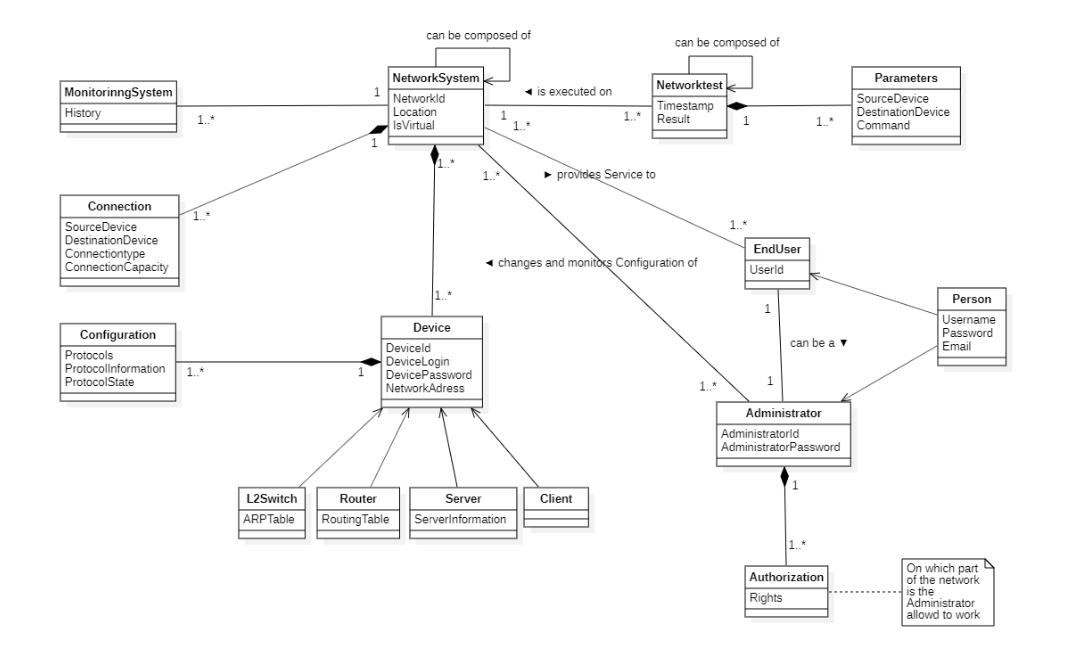
\includegraphics[scale = 0.825]{\vorlagenOrdner/Bilder/DomainModell}
	\newpage	
\end{landscape}


	\subsection{Prosa}
	Ein Netzwerk (Network System) setzt sich aus mindestens zwei Geräten (Device) und Verbindungen dazwischen (Connection) zusammen.
	Es kann auch mehrere Teilnetzwerke in sich vereinen, z.B die beiden Netzwerke aus Haupt- und Nebengebäude ergeben das gesammte Firmennetzwerk.
	Das Netzwerksystem kann auch in Virtueller Form aufgebaut sein, Beispielsweise als Netz von virtuellen Routern auf einem Server.
	Ein Device kann in die vier Kategorien Switch, Router (Level-3-Switch), Server und Client eingeteilt werden und hat eine oder mehrere Konfigurationen.
	Beispielsweise kann ein Router das OSPF (Open Shortest Path First) Protokoll und zusätzlich als Fallback statische Routen konfiguriert haben.

	Geräte haben eine Identifikation, ein Gerätelogin und -passwort und eine Addresse innerhalb des Netzwerkes.
	Die Konfiguration der Geräte setzt sich zusammen aus dem Protokoll, dessen Informationen und dem Zustand, in dem das Gerät mit dem Protokoll gerade ist.

	Es ist möglich, dass ein Netzwerksystem ein Monitoring System hat, das die Zustände zur Laufzeit überwacht, z.B. Welche Verbindungen gerade aktiv sind und wieviele Client auf dem Netzwerksystem angemeldet sind.
	Das Monitoring speichert auch vergangene Daten in einer Historie, so dass vergangene Zustände mit dem aktuellen Zustand verglichen werden können.

	Netzwerktests, wie sie von Netzwerk-Technikern auf dem Netzwerk ausgeführt werden, haben Parameter und können aus weiteren Tests zusammengesetzt sein. 
	Ein umfangreicher Systemtest kann aus mehreren Ping-Tests bestehen.
	Ein Netzwerktest umfasst einen Zeitstempel, um die genaue Durchführungszeit ermitteln zu können und hat ein Resultat, üblicherweise "bestanden" oder "durchgefallen".
	Die Parameter eines Netzwerktests sind üblicherweise ein Befehl (Ping, Traceroute etc.) und ein Source- und/oder Destination-Device.

	Auf dem Netzwerksystem arbeiten verschiedene Personen. 
	Jede Person benötigt einen Usernamen, ein Passwort und eine E-Mail-Addresse, um sich gegenüber dem Neztwerk zu authentifizieren.
	Diese können in User und Administratoren eingeteilt werden. 
	Usern werden Services vom Netzwerk wie Internet oder Serverzugriff angeboten, und sie haben eine UserID, mit der sie das Netzwerk erkennt.
	Administratoren können die Konfiguration des Netzwerks einsehen und verändern. 
	Zusätzlich zum regulären Login haben sie einen Administratorzugriff, der aus einer ID und einem Admin-Passwort besteht.
	Dazu benötigen sie eine Authorisierung, um auf dem Netzwerksystem zu arbeiten.

\begin{landscape}
	\section{Klassendiagramm}
	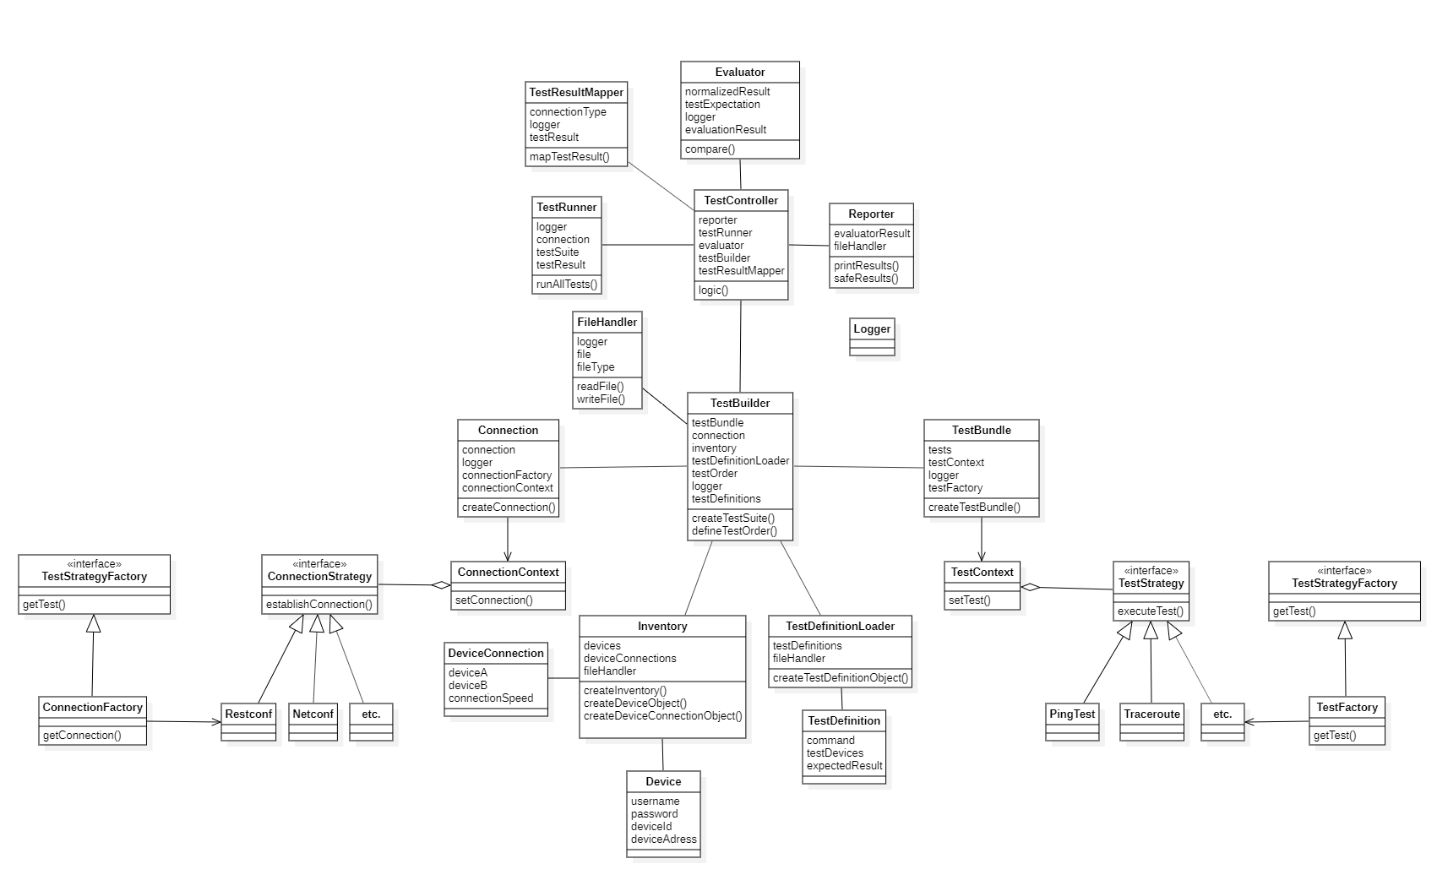
\includegraphics[scale = 0.6]{\vorlagenOrdner/Bilder/Klassendiagramm}
	\newpage	
\end{landscape}


	\subsection{Beschreibungen}

	\subsubsection{TestController}
	Der TestController ist das Kernstück des Programms. 
	Er beinhaltet die Main-Methode und steuert den Ablauf des Programms. 
	Vom TestController werden der TestRunner, der TestBuilder, der Evaluator und der Reporter instanziert und er ist zuständig für die Kommunikation zwischen diesen Komponenten.
	
	\begin{tabularx}{\textwidth}{lX}
		\toprule
			Komponenten & Beschreibung \\
		\midrule
			reporter & Referenz auf das Reoprter-Objekt \\
			testRunner & Referenz auf das TestRunner-Objekt \\
			evaluator & Referenz auf das Evaluator-Objekt \\
			testBuilder & Referenz auf das TestBuilder-Objekt \\
		\midrule
			logic() & Methode, die für die Programmausführung sämtliche referenzierten Komponenten instanziert und deren Funktionalität in der korrekten Reihenfolge ausführt.\\
		\bottomrule
	\end{tabularx}

	\subsubsection{TestRunner}
	Der TestRunner führt die ihm vom Controller mitgeteilten Tests gemäss der in der TestSuite angegebenen Parameter aus. 
	Die zu verwendende Netzwerkschnittstelle (Restconf, Netconf, SSH etc.) wird ihm ebenfalls vom Controller mitgeteilt.
	Die Resultate der Netzwerktests gibt er dem TestController in form von Rückgabewerten zurück.

	\begin{tabularx}{\textwidth}{lX}
		\toprule
			Komponenten & Beschreibung \\
		\midrule
			logger & Referenz auf das Logger-Objekt \\ 
			connection & Referenz auf das Connection-Objekt \\
			testSuite & Collection von Testspezifikationen, welche Tests sollen auf welchen Netzwerkkomponenten in welcher Reihenfoge ausgeführt werden. \\
			testResult & Resultat der Netzwerktests die dem Controller nach abarbeiten aller Tests zurückgegeben werden. \\			
		\midrule
			runAllTests() & Methode, die die in der Testsuite spezifiszierten Tests auf der in der Connection spezifiszierten Netzwerkschnittstelle ausführt. \\
		\bottomrule
	\end{tabularx}
	\newpage

	\subsubsection{Reporter}
	Der Reporter schreibt die Testergebnisse der fertig ausgeführten Tests auf die Konsole/Benutzeroberfläche und erstellt ein Testprotokoll, welches er über den FileHandler im Directory abspeichert.

	\begin{tabularx}{\textwidth}{lX}
		\toprule
			Komponenten & Beschreibung \\
		\midrule
			evaluationResult & Die Ergebnisse des Evaluators, wie der Soll- Ist-Vergleich der Tests abgelaufen ist. \\
			fileHandler & Referenz auf das FileHandler-Objekt. \\	
		\midrule
			printResults() & Methode die die Testergebnisse auf der Konsole ausgibt. \\
			safeResults() & Methode, die über den FileHandler die Testergebnisse in einem File im Directory abspeichert. \\
		\bottomrule
	\end{tabularx}

	\subsubsection{Evaluator}
	Der Evaluator vergleicht die ihm vom Controller mitgeteilten Testresultate mit den Testerwartungswerten und evaluiert, ob die Tests bestanden sind oder nicht.

	\begin{tabularx}{\textwidth}{lX}
		\toprule
			Komponenten & Beschreibung \\
		\midrule
			testRunnerResult & Ergebnisse der auf dem Netzwerk vom Runner ausgeführten Tests. \\
			testExpectation & Zu erwartende Ergebnisse für einen spezifischen Test der Testsuite. \\
			logger & Referenz auf das Logger-Objekt. \\
			evaluationResult & Resultat des Soll-Ist-Vergleichs, welches dem Controller zurückgegeben wird.\\
		\midrule
			compare() & Methode, die testRunnerResult mit testExpectation vergleicht und entscheidet, ob der Test erfolgreich war oder gescheitert ist. \\
		\bottomrule
	\end{tabularx}
	\newpage

	\subsubsection{FileHandler}
	Der FileHandler ist eine Utility-Klasse, die für das einlesen und schreiben von Daten aus dem Programm in das Directory zuständig ist.
	
	\begin{tabularx}{\textwidth}{lX}
		\toprule
			Komponenten & Beschreibung \\
		\midrule
			logger & Referenz auf das Logger-Objekt. \\
			file & Pfad zu dem zu lesenden/schreibenden File. \\
			fileType & Typ des Files, YAML, XML, JSON usw. \\
		\midrule
			readFile() & Methode, die ein vorgegebenes File öffnet und deren Inhalt in das Programm einliest. \\
			writeFile() & Methode, die einen vorgegebenes Text aus dem Programm in ein File im Directory schreibt. \\
		\bottomrule
	\end{tabularx}

	\subsubsection{Testbuilder}
	Der Testbuilder ist für die zusammenstellung der Tests verantwortlich. 
	Er instanziert einen TestDefinitionLoader, der aus dem TestDefinitionsDirectory, wo mehrere Files mit TestDefinitionen gespeichert sind, die einzelnen TestDefinitionen ausliest.
	Dann holt er sich aus dem Inventory die Devices und deren Connections. 
	Die TestDefinitionen attributisiert er mit den in der TestStrategy definierten Tests erstellt mit den Parametern aus dem Inventar das TestBundle. 
	Hier kann vom Benutzer auch die Auswahl der einzelnen Tests, welche durchgeführt werden sollen, sowie die Durchführungsreihenfolge festgelegt werden.
	Die Connection spezifiziert die konkrete Netzwerkschnittstelle, über welche die Netzwerktests vom Runner dann durchgeführt werden sollen.

	\begin{tabularx}{\textwidth}{lX}
		\toprule
			Komponenten & Beschreibung \\
		\midrule
			testBundle & Collection von Tests mit Parametern für die Ausführung als Referent auf ein TestBundle-Objekt. \\
			connection & Referenz auf das Connection-Objekt. \\
			inventory & Referenz auf das Inventory-Objekt. \\
			testDefinitionLoader & Referenz auf ein TestDefinitionLoader-Objekt.\\
			testOrder & Definition, in welcher Reihenfolge die Tests ausgeführt werden sollen. \\
			logger & Referenz auf das Logger-Objekt.  \\
			testDefinitions & Collection mit Referenzen auf TestDefinition-Objekte. \\
		\midrule
			createTestSuite() & Methode, die aus den destDefinitionen, dem Inventar und der Testreihenfolge eine TestSuite erstellt. \\
			defineTestOrder() & Methode, die die Testreihenfolge vom Softwareuser einstellen lassen kann. \\
		\bottomrule
	\end{tabularx}
	\newpage

	\subsubsection{TestBundle}
	Das TestBundle ist dafür zuständig, gemäss der TestDefinitionen die Tests zusammenzustellen. 
	Dazu wird ein TestContext und eine TestFactory instanziert und damit die Tests ausgewählt und instanziert.

	\begin{tabularx}{\textwidth}{lX}
		\toprule
			Komponenten & Beschreibung \\
		\midrule
			tests & Collection von Tests, die von der TestFactory instanziert wurden und dem TestBuilder als Rückgabewert zurückgegeben wird. \\
			testContext & Referenz auf das TestContext-Objekt. \\
			logger & Referenz auf das Logger-Objekt. \\
			testFactory & Referenz auf das TestFactory objekt. \\
		\midrule
			createTestBundle() & Methode, die aus den TestDefinitionen über eine TestFactory die konkreten Tests auswählt und in einer Collection zusammenfasst. \\
		\bottomrule
	\end{tabularx}

	\subsubsection{TestContext}
	Der TestContext wird benötigt, um unter Anwendung des Strategy-Pattern die Auswahl der Tests durchzuführen.
	Die Methode setText() ruft dabei die Facktory auf und instanziert die konkreten Tests.

	\subsubsection{TestStrategy}
	Das TestStrategy-Interface dient als Basis für die konkreten implementationen der Tests. 
	Das Interface gibt den Test-Classes dafür die benötigte Funktionalität vor, die wiederum von den konkreten Tests implementiert werden müssen.
	Die ExecuteTest() Methode ist ein Beispiel für eine solche Funktionalität.

	\subsubsection{TestFactory}
	Die TestFactory ist die Anwendung des Factory Method pattern, welches es den Tests erlaubt, instanziert zu werden, ohne dass sich diese selbst um die Instanzierungslogik kümmern müssen.
	Die Factory entscheidet dabei, welche Tests für welche Definitionen instanziert werden müssen und instanziert diese konkreten Tests mit der getTest() Methode.

	\subsubsection{TestDefinitionLoader}
	Der TestDefinitionLoader ist dafür zuständeg, die TestDefinitionen aus dem Directory zu laden und als einzelne TestDefinitionen zu instanzieren.
	
	\begin{tabularx}{\textwidth}{lX}
		\toprule
			Komponenten & Beschreibung \\
		\midrule
			testDefinitions & Collection von TestDefinitionen, die dem TestBuilder als Rückgabewerte zurückgegeben werden. \\
			fileHandler & Referenz auf das FileHandler-Objekt. \\
		\midrule
			createTestDefinitionObject & Methode, die die TestDefinitionen aus dem FileSystem ausliest und TestDefinition-Objekte für jede Definition instanziert. \\
		\bottomrule
	\end{tabularx}

	\subsubsection{Inventory}
	Das Inventory ist diejenige Klasse, die im Programm die einzelnen Geräte und deren Verbindungen untereinander verwaltet. 
	Sie liest dazu aus dem FileSystem die spezifizierten Devices und DeviceConnections ein und instanziert Klassen, um diese als Collection dem TestBuilder zurückzugeben.

	\begin{tabularx}{\textwidth}{lX}
		\toprule
			Komponenten & Beschreibung \\
		\midrule
			devices & Collection der eingelesenen Geräte.\\
			deviceConnection & Collection der Geräteverbindungen. \\
			fileHandler & Referenz auf das FileHandler-Objekt.\\
		\midrule
			createInventory() & Methode, die das Inventar erstellt. \\
			createDeviceObject & Methode, die aus dem FileSystem die einzelnen Devices ausliest und für jedes ein Device-Objekt erstellt. \\
			createDeviceConnectionObject & Methode, die aus dem FileSystem die Geräteverbindungen ausliest und für jede Verbindung ein deviceConnection-Objekt erstellt.\\
		\bottomrule
	\end{tabularx}
	\newpage

	\subsubsection{Connection}
	Die Connection-Klasse spezifiziert die Netzwerk-Schnittstelle, die für die Verbindung zwischen dem Programm und des zu Testenden Netzwerks verwendet werden soll.
	Für die Auswahl und Instanzierung wird eine ConnectionFactory verwendet und die Verbindungen lassen sich mittels einem Strategy-Pattern auswählen.

	\begin{tabularx}{\textwidth}{lX}
		\toprule
			Komponenten & Beschreibung \\
		\midrule
			connection & Ausgewählte Netzwerkschnittstelle, die dem TestBuilder als Rückgabewert geliefert wird. \\
			logger & Referenz auf das Logger-Objekt. \\
			connectionFactory & Referenz auf das ConnectionFactory-Objekt. \\
			connectionContext & Referenz auf das ConnectionContext-Objekt. \\
		\midrule
			createConnection() & Methode, die aufgrund der Parameter der Devices eine mögliche Netzwerkschnittstelle auswählt.\\
		\bottomrule
	\end{tabularx}

	\subsubsection{ConnectionContext}
	Anwendung des Strategy Pattern für die Netzwerkschnittstelle. 
	Der ConnectionContext hält eine Referenz auf das konkrete Schnittstellen-Objekt.

	\subsubsection{ConnectionFactory}
	Anwendung des Facktory-Pattern auf die Netzwerkschnittstelle.
	Die Factory ist zuständig für die Instanzierung der konkreten Schnittstelle, mit der das Programm die Neztwerkumgebung testet.

	\subsubsection{Logger}
	Der Logger wird verwendet, um wichtiche Informationen zentral zu speichern. 
	Diese Informationen betreffen nur den Systemzustand des zu entwickelnden Systems.
	Der Loger speichert Fehlermeldungen, erfolgsbenachrichtigungen und weitere Informationen, die es einem Entwickler erlauben, unerwartetes Verhalten der Software besser zu verstehen.
	

	\subsection{Konzepte}


\begin{landscape}
	\section{Systemsequenzdiagramme}
		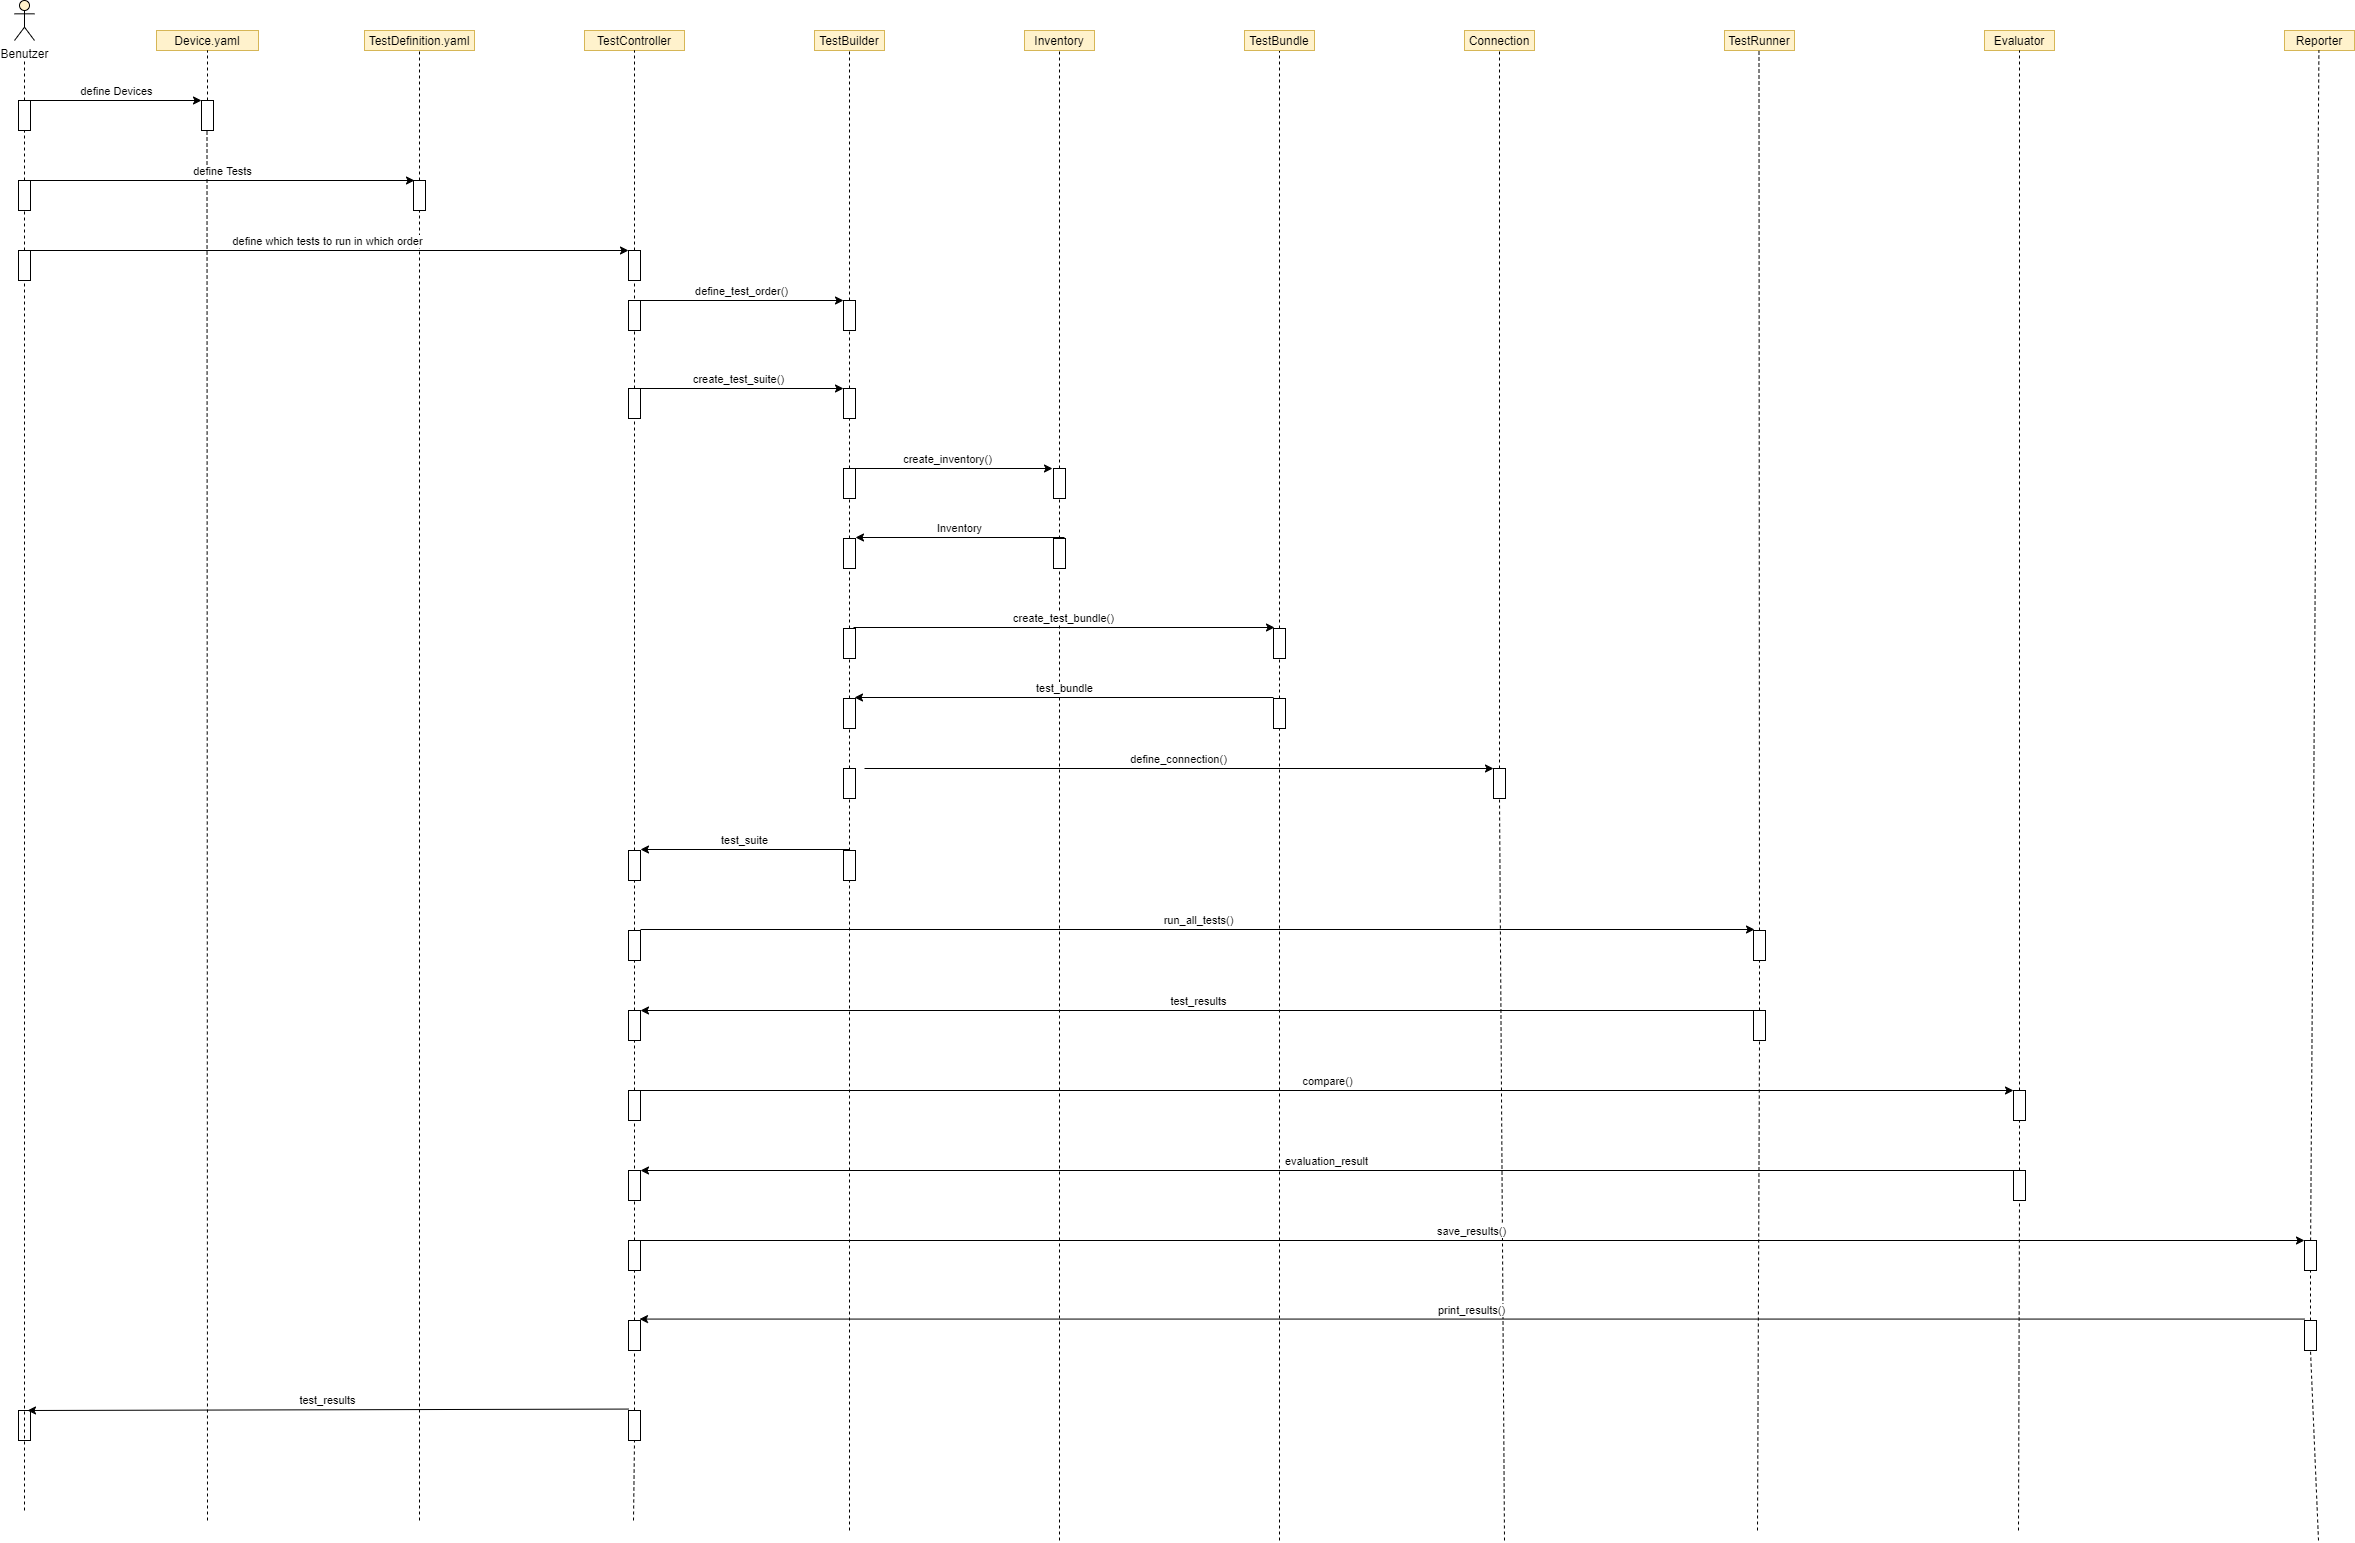
\includegraphics[scale=0.25]{\vorlagenOrdner/Bilder/SystemSSD}
		\newpage
\end{landscape}
	
	\subsection{TestBundle}
		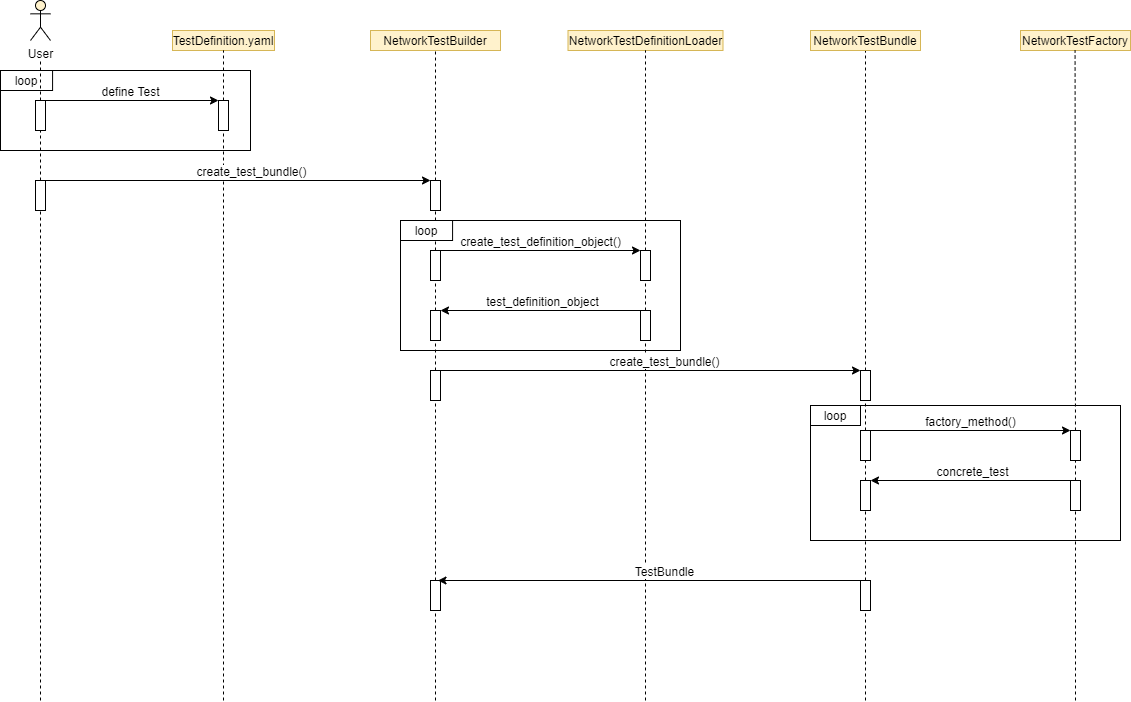
\includegraphics[scale=0.35]{\vorlagenOrdner/Bilder/TestSSD}
	
	\subsection{Inventar}
		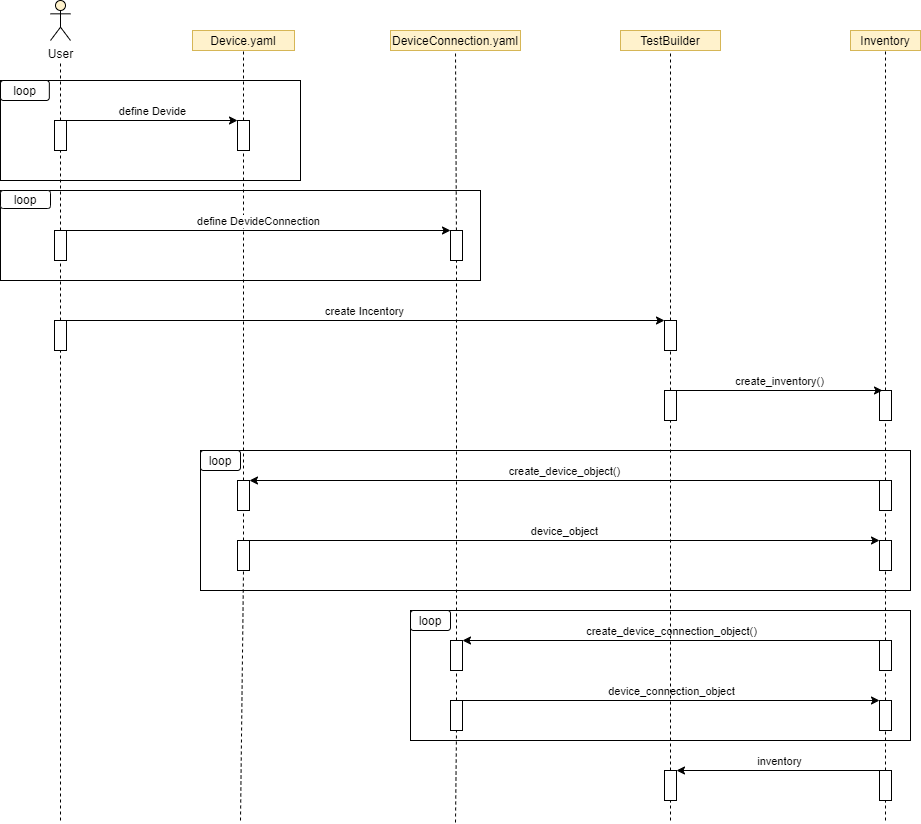
\includegraphics[scale=0.5]{\vorlagenOrdner/Bilder/InventorySSD}

	\subsection{Connection}
		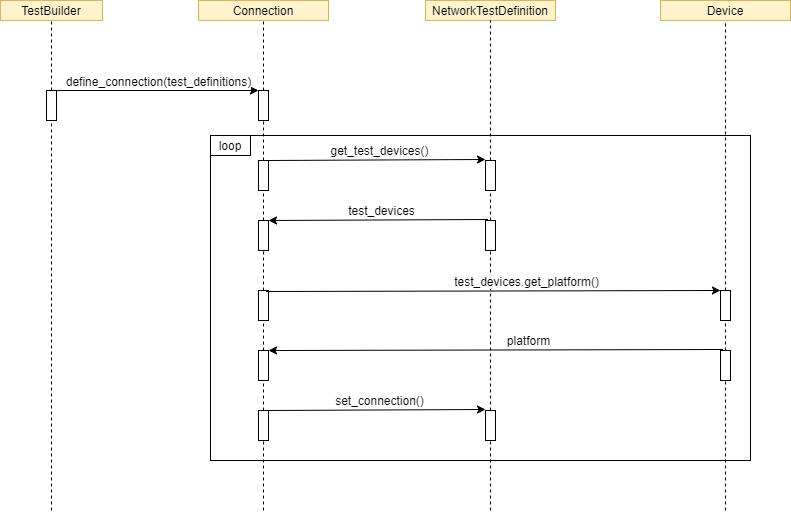
\includegraphics[scale=0.5]{\vorlagenOrdner/Bilder/ConnectionSSD}


\end{document}